\subsection{Einleitung}
Zahlreiche Dienste wie Dropbox, Google Drive, iCloud, Microsoft OneDrive und Box
bieten ihren Kunden kostenlosen Cloudspeicher an.
Der Vorteil bei der Verwendung solcher Dateisynchronisationsdienste liegt in der
Einfachheit, mit der diese Dienste Datenbestände auf mehreren Geräten synchron
halten.

Besonders bei Verwendung eines Laptops in der Schule und eines zweiten Rechners
Zuhause ist die Anmeldung bei einem dieser Anbieter hilfreich.
Statt Dateien mühsam über externe Speichermedien wie USB-Sticks kopieren zu
müssen, kann ein Synchronisationsclient des Anbieters installiert werden, der
neue und geänderte Dateien von einem Gerät automatisch in die \gls{filecloud}
lädt und anschließend auf das zweite Gerät synchronisiert.

Die meisten Cloudspeicher sind so aufgebaut, dass die Daten der Nutzer zentral
und unverschlüsselt auf Servern des Anbieters gespeichert werden.
Dieses Modell ist zwar das simpelste, effizienteste und am einfachsten
umzusetzen, birgt aber Risiken für die Privatsphäre der Nutzer.

Durch die zentrale Speicherung der Daten entsteht ein einziger Angriffspunkt,
der, wenn ein Angriff erfolgreich oder ein Fremdzugriff auf einem anderen Weg
möglich ist, den Zugang zum gesamten System und damit zu den Daten aller Nutzer
erlaubt.
Der Verzicht auf die Verschlüsselung der Daten ermöglicht es einem Angreifer
außerdem, die Daten vollständig auszuwerten.

\sblitg verfolgt statt einer klassischen Client-Server-Infrastruktur einen
vollständig dezentralen Ansatz in Kombination mit starker Verschlüsselung,
wodurch es keinen zentralen Angriffspunkt mehr gibt, der die Privatsphäre der Nutzer gefährdet.

\subsection{Funktionsweise üblicher Dateisynchronisationsdienste}
\subsubsection{Allgemein}
Die Erläuterung der Funktionsweise üblicher Dateisynchronsationsdienste soll beim
Verstehen der grundsätzlichen Idee von \sblit helfen, da diese auf den
sicherheitsbezogenen Problemen basiert, die mit der Speicherung von Daten auf einer
zentralen Stelle einhergehen.

Übliche Dateisynchronisationsdienste bauen auf einer Client-Server-Struktur auf.
Hierbei werden Dateien auf zentrale Server des betreibenden
Unternehmens übertragen, zwischengespeichert, verwaltet und schließlich
synchronisiert.

\subsubsection{Szenario}
In der Schule wird ein Übungsprotokoll geschrieben. Wird die Übung nicht
fertiggestellt, muss sie zu Hause fertiggestellt werden.

Beim Erstellen und Bearbeiten des Übungsprotokolls auf dem Schulrechner
wird eine Kopie dieser Datei auf die vom Betreiber zur Verfügung gestellten
\gls{filecloud} beziehungsweise dessen Server hochgeladen und dort gespeichert.
Der Sender behält dabei die Originaldatei (\figurelink{dropbox_upload}).
\begin{figure}[htb]
	\centering
  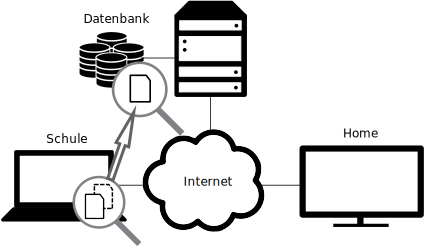
\includegraphics[]{images/dropbox_upload}
  \caption{Üblich gehandhabtes Uploaden einer Datei}
	\label{dropbox_upload}
\end{figure}

Der Schulrechner wird heruntergefahren, zu Hause wird der Heimrechner hochgefahren. Die Synchronisations-Software wird,
sobald gestartet, über die Änderungen in der \gls{filecloud} informiert und aktualisiert den lokalen Datenbestand, in
diesem Fall durch Herunterladen des neu angelegten Übungsprotokolls vom Server (\figurelink{dropbox_download}).

\begin{figure}[htb]
	\centering
  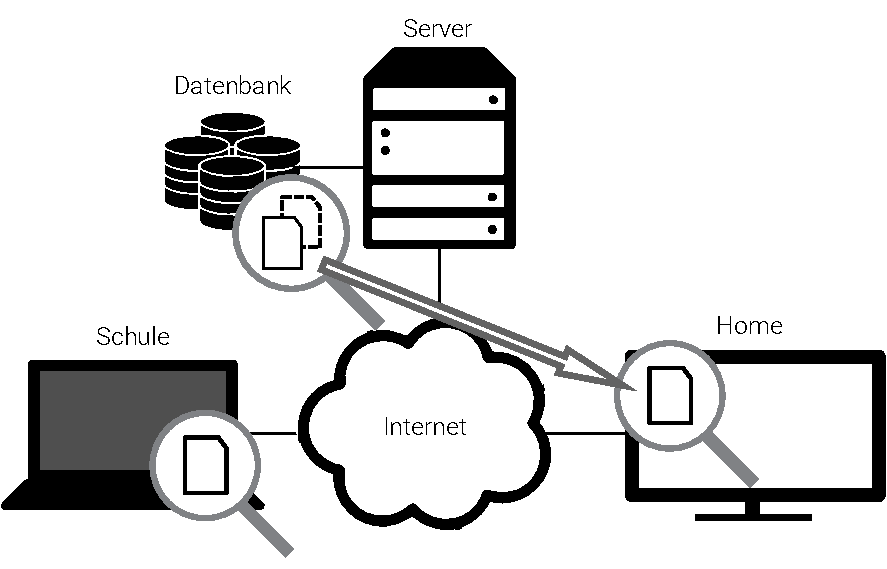
\includegraphics[]{images/dropbox_download}
  \caption{Üblich gehandhabtes Downloaden einer Datei}
	\label{dropbox_download}
\end{figure}

Das Übungsprotokoll hat nach dem Synchronisationsvorgang auf dem Heim-PC
den gleichen Inhalt wie die Datei auf dem Schulrechner, da es sich um die selbe Version
handelt. Würde das Übungsprotokoll nun auf dem Heim-PC bearbeitet werden, würde
die neue Version analog dazu zuerst auf den Server geladen werden und vom Server
aus auf die anderen Rechner synchronisiert werden.
